\noindent In the first session we we will define our \textbf{\emph{mission}} and evaluate why R is the tool choice that enables us to achieve our mission. Moreover, we will present an overview of the \textbf{\emph{concepts}} for programming with R. Then we will introduce the ``R environment'' and provide instructions for setting up \textbf{\emph{RStudio}}. Furthermore, we will explain different features of the RStudio environment so that the reader gets accustomed to working with RStudio. Finally, we will demonstrate how to read data sets, organized in tabular format, into R and take the first steps towards processing and transforming such data.
Throughout this manual, the participant will come across the following two icons

\begin{minipage}[ht]{0.2\linewidth}
    
\includegraphics[width=2\baselineskip]{./viz/icons/Think.png}  
\end{minipage}%
\begin{minipage}[ht]{0.75\linewidth}
\emph{This icon urges the reader to think about the question that has been asked and such questions will be the main discussion points during sessions.}
\end{minipage}

\begin{minipage}[ht]{0.2\linewidth}
    
\includegraphics[width=2\baselineskip]{./viz/icons/Homework.png}  
\end{minipage}%
\begin{minipage}[ht]{0.75\linewidth}
\emph{This icon will be associated with an assignment and the participants are expected to work on these.}
\end{minipage}


\begin{minipage}[ht]{0.2\linewidth}
    
\includegraphics[width=2\baselineskip]{./viz/icons/Warning.png}  
\end{minipage}%
\begin{minipage}[ht]{0.75\linewidth}
\emph{This icon will be used when we want the reader to pay attention to a particular idea.}
\end{minipage}

\clearpage
%==========================
\section{The Mission}
%==========================
\begin{mdframed}[backgroundcolor=cyan!10]
\par\noindent{
{\centering\textbf{\emph{\Huge ``Data Exploration''}} \\}
\vspace{\baselineskip}
\textbf{Data Exploration} entails the following actvities:
\begin{enumerate}
      \item Formulation of  meaningful questions
      \item Organization of data in a way to answer the questions
\end{enumerate}
}
\end{mdframed}

\begin{minipage}[ht]{0.2\linewidth}
    
\includegraphics[width=2\baselineskip]{./viz/icons/Homework.png}  
\end{minipage}%
\begin{minipage}[ht]{0.75\linewidth}
\emph{Explore} the dataset in exercise1.csv
\end{minipage}

\subsection{Data and Society}
\begin{figure}[ht]
 \centering
    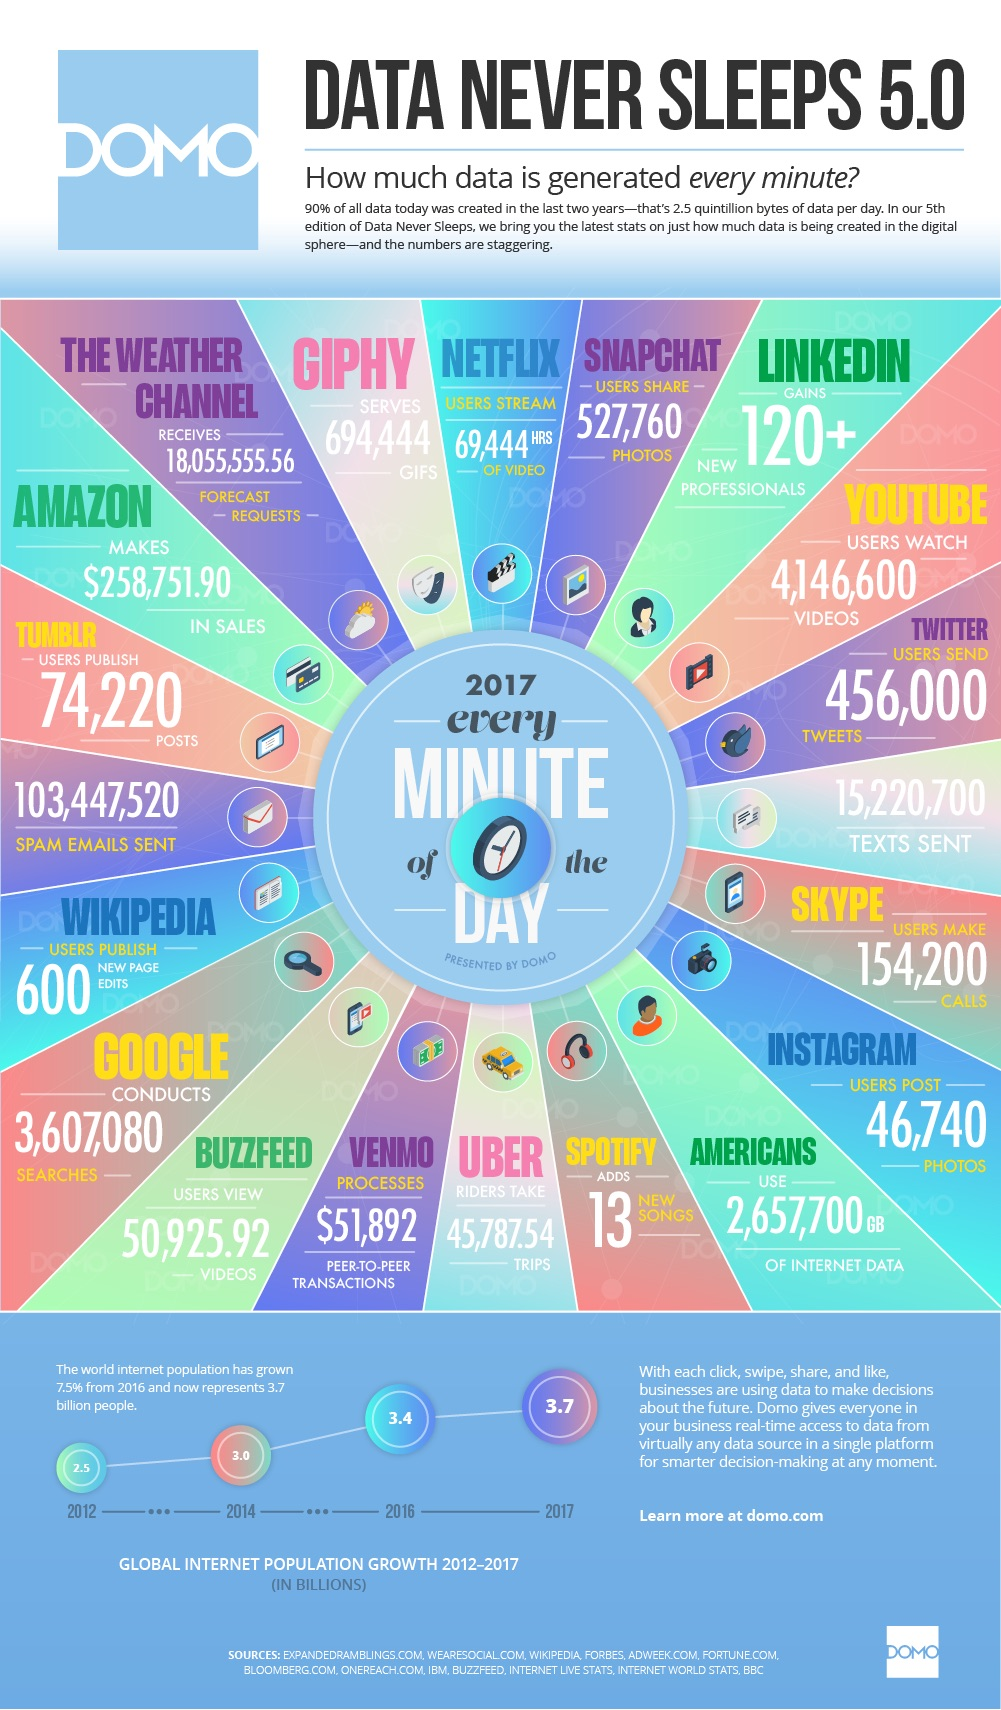
\includegraphics[width = 8 cm]{./viz/ext/dataeachday2017.jpg}
\end{figure}
\begin{figure}[ht]
 \centering
    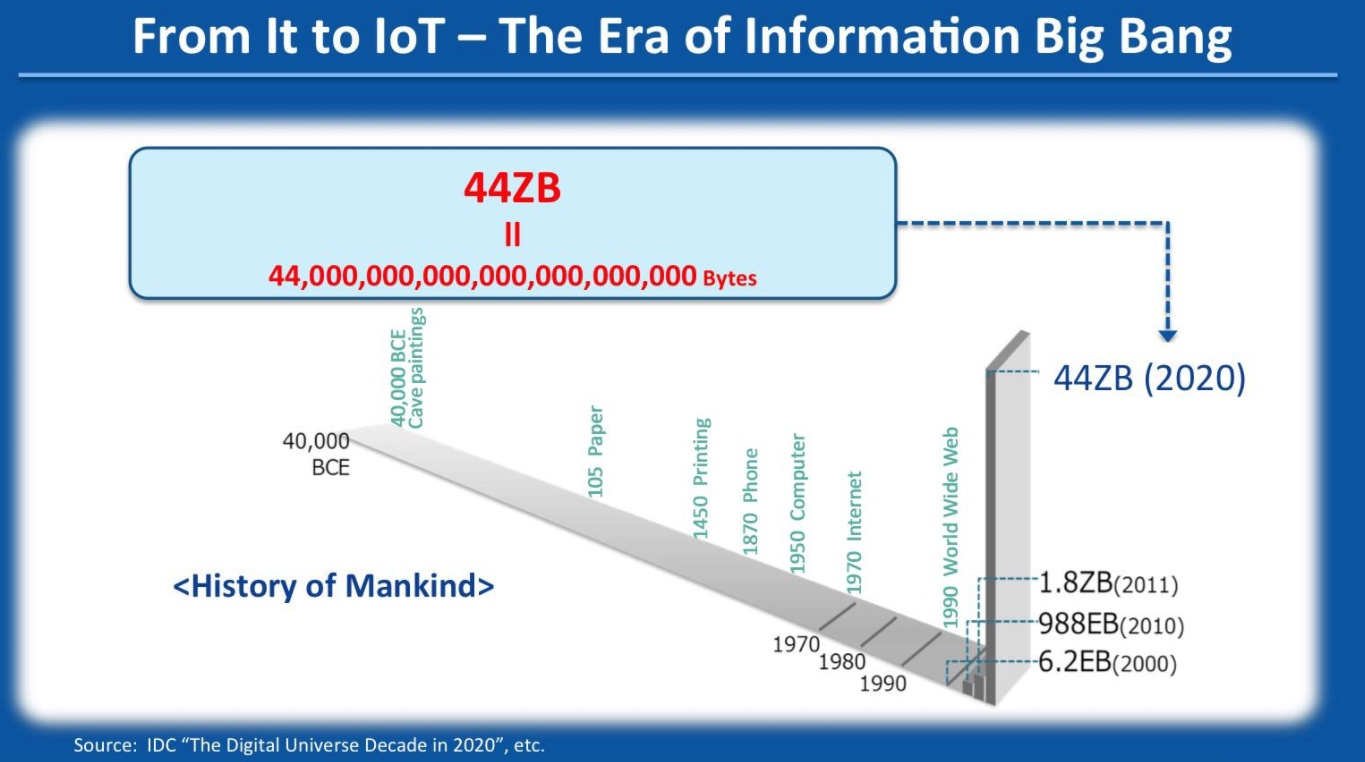
\includegraphics[width = 10 cm]{./viz/ext/DataVolumesVSHumanHistory.jpeg}
\end{figure}

\begin{minipage}[ht]{0.2\linewidth}
    
\includegraphics[width=2\baselineskip]{./viz/icons/Think.png}  
\end{minipage}%
\begin{minipage}[ht]{0.75\linewidth}
It is true that data is ubiqutous to modern society and is being generated at an unprecedented scale at high \textbf{\emph{volumes}}, \textbf{\emph{velocity}} and \textbf{\emph{variety}} (the \textbf{3V's}). Try categorizing each of the data source in the infographic
\begin{itemize}
  \item into one of the \textbf{3V's}  
  \item \textbf{\emph{high noise-to-signal}} ratio source v/s \textbf{\emph{low noise-to-signal}} ratio source
  \item sources where high volume \textbf{\emph{correlates}} to better insights 
\end{itemize}
\end{minipage}

\subsection{Stages of Data Exploration}
\begin{mdframed}[backgroundcolor=cyan!10]
\par\noindent{
The various stages of data exploration can be classified into the following:
\begin{enumerate}
  \item Accessing Data
  \item Transforming Data
  \item Generating Summaries of the Data
  \item Making Predictions on the Data
  \item Communicating Findings
\end{enumerate}
}
\end{mdframed}

\begin{minipage}[ht]{0.2\linewidth}
    
\includegraphics[width=2\baselineskip]{./viz/icons/Think.png}  
\end{minipage}%
\begin{minipage}[ht]{0.75\linewidth}
Which \emph{Stages of Data Exploration} did you apply while exploring the dataset in exercise1.csv
\end{minipage}

\newpage
\subsection{Software of Data Exploration}
\begin{mdframed}[backgroundcolor=cyan!10]
\par\noindent{
{\centering\textbf{\emph{\Large ``Trustworthy, Flexible and Efficient Software: The Prime Directives''}} \\}
\vspace{\baselineskip}
\noindent The task of data exploration requires a tool that allows a user to ask meaningful questions about their applications quickly and flexibly. A wide range of techniques is needed to facilitate stages 1-4 of data exploration thereby requiring the data exploration tool to be flexible. Moreover, the tool should be able to provide answers to the questions asked ``\emph{within an acceptable timeframe}''. The \textbf{3V's}, and the questions that are posed on the data, require complex transformations and computations on the data, whose correctness cannot be often verified by direct observation of the results in stage 5. Therefore, it is imperative that the underlying implementations of the transformations and computaions (which is often \textbf{\emph{encapsulated}}) are correct.
}
\end{mdframed}

\begin{minipage}[ht]{0.2\linewidth}
    
\includegraphics[width=2\baselineskip]{./viz/icons/Think.png}  
\end{minipage}%
\begin{minipage}[ht]{0.75\linewidth}
How does Microsoft Excel provide \textbf{\emph{Abstraction via Encapsulation}}. Think of an example there the trustworthiness comes into play.
\end{minipage}

\begin{minipage}[ht]{0.2\linewidth}
    
\includegraphics[width=2\baselineskip]{./viz/icons/Warning.png}  
\end{minipage}%
\begin{minipage}[ht]{0.75\linewidth}
It is extremely hard to achieve \emph{trustworthiness}, \emph{flexibility} and \emph{efficiency} at the same time. As you go ahead in the course try to identify trade-offs between the three directives in R.  
\end{minipage}


\newpage
%==========================
\section{Why R?}
%==========================
\noindent Before delving into the question of \emph{why R?}, let us first take a look at how R fares with respect to to its competitors.The following two plots show the results of two surveys conducted in the year 2017. The first survey was conducted by O'Rielly in Europe and shows the popularity of different tools among data analysts/scientists. The second plot shows the result of a similar survey, conducted worlwide, by Kaggle. 
    \begin{figure}[ht] % Figure to demonstrate popularity of R in O'Rielly surveys
      \centering
      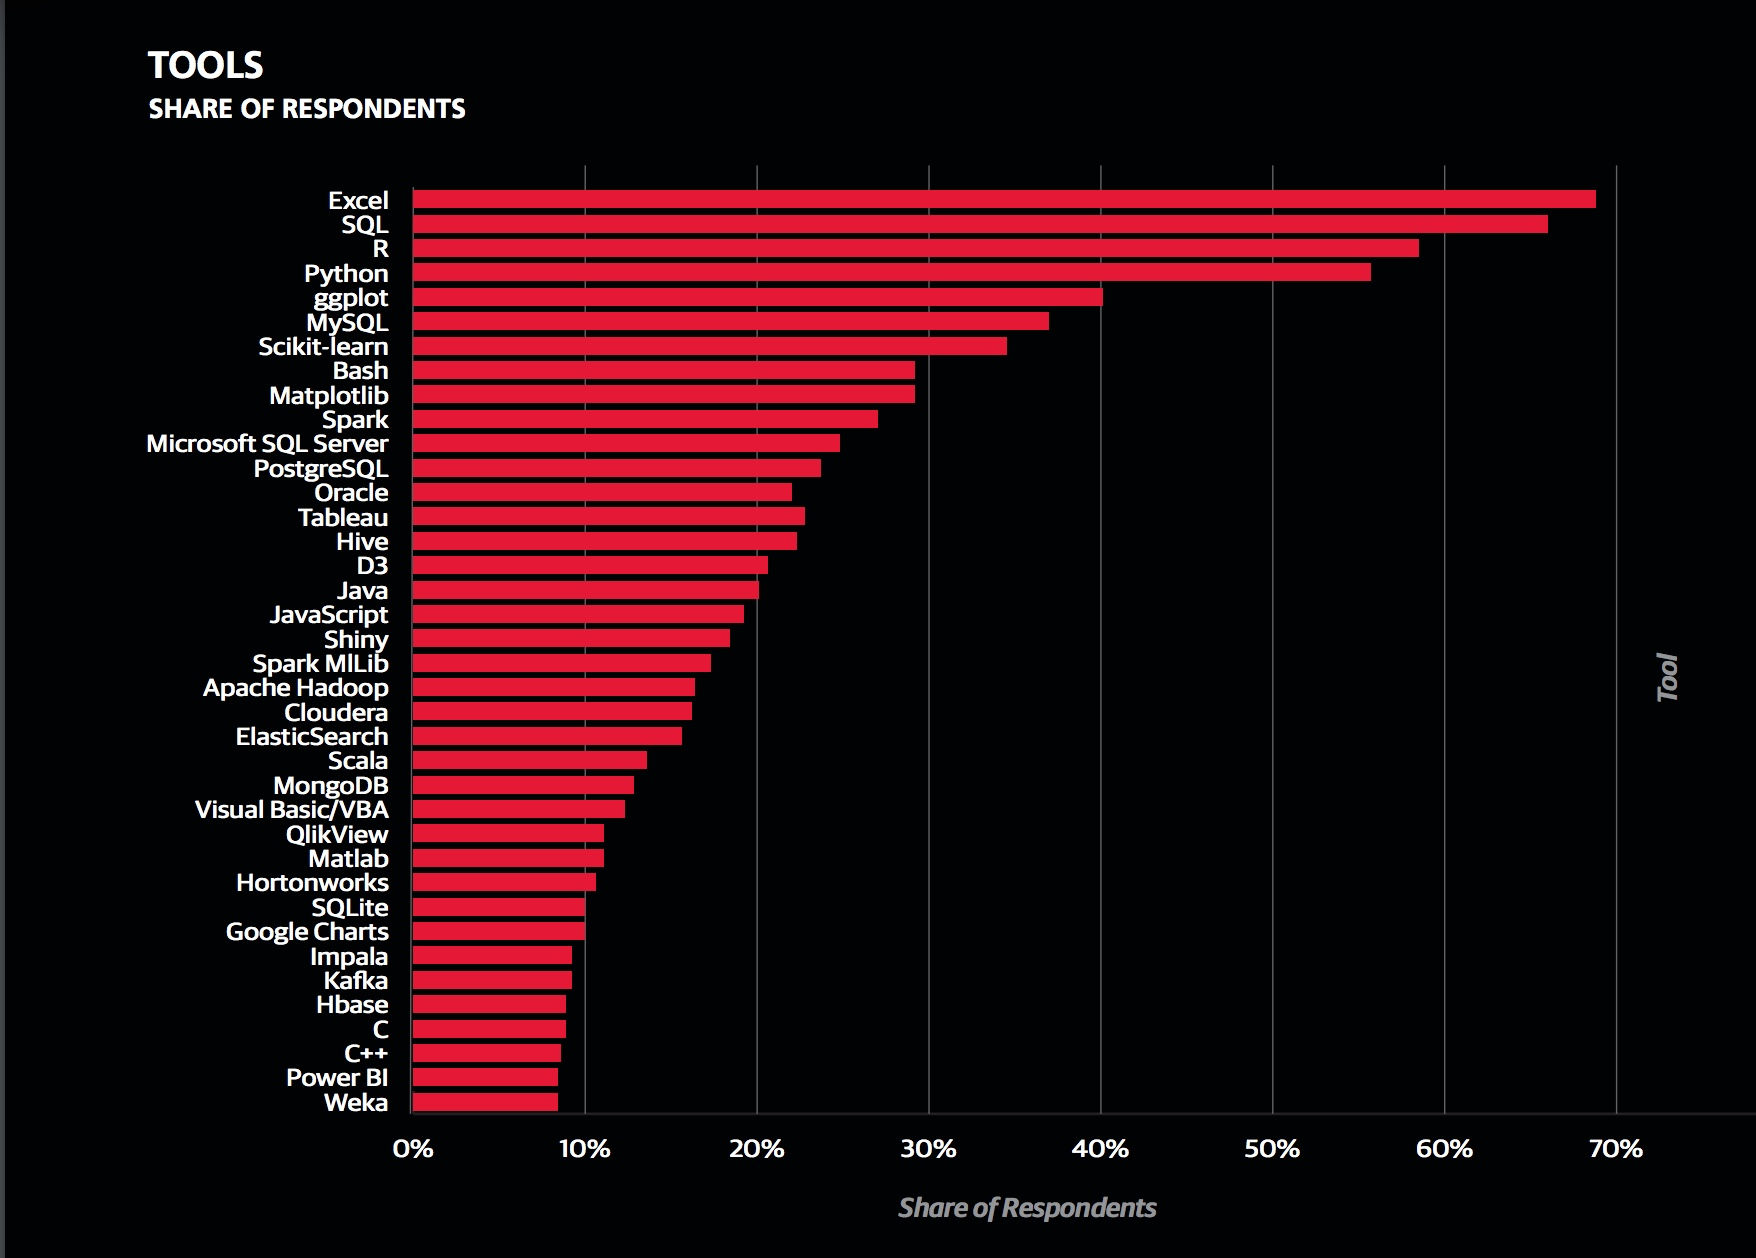
\includegraphics[width = 10 cm]{./viz/ext/OR_DS_Tools_Survey.jpeg}
    \end{figure}
    % Figure to demonstrate popularity of R in Kaggle surveys
    \begin{figure}[ht] % Figure to demonstrate popularity of R in O'Rielly surveys 
      \centering
      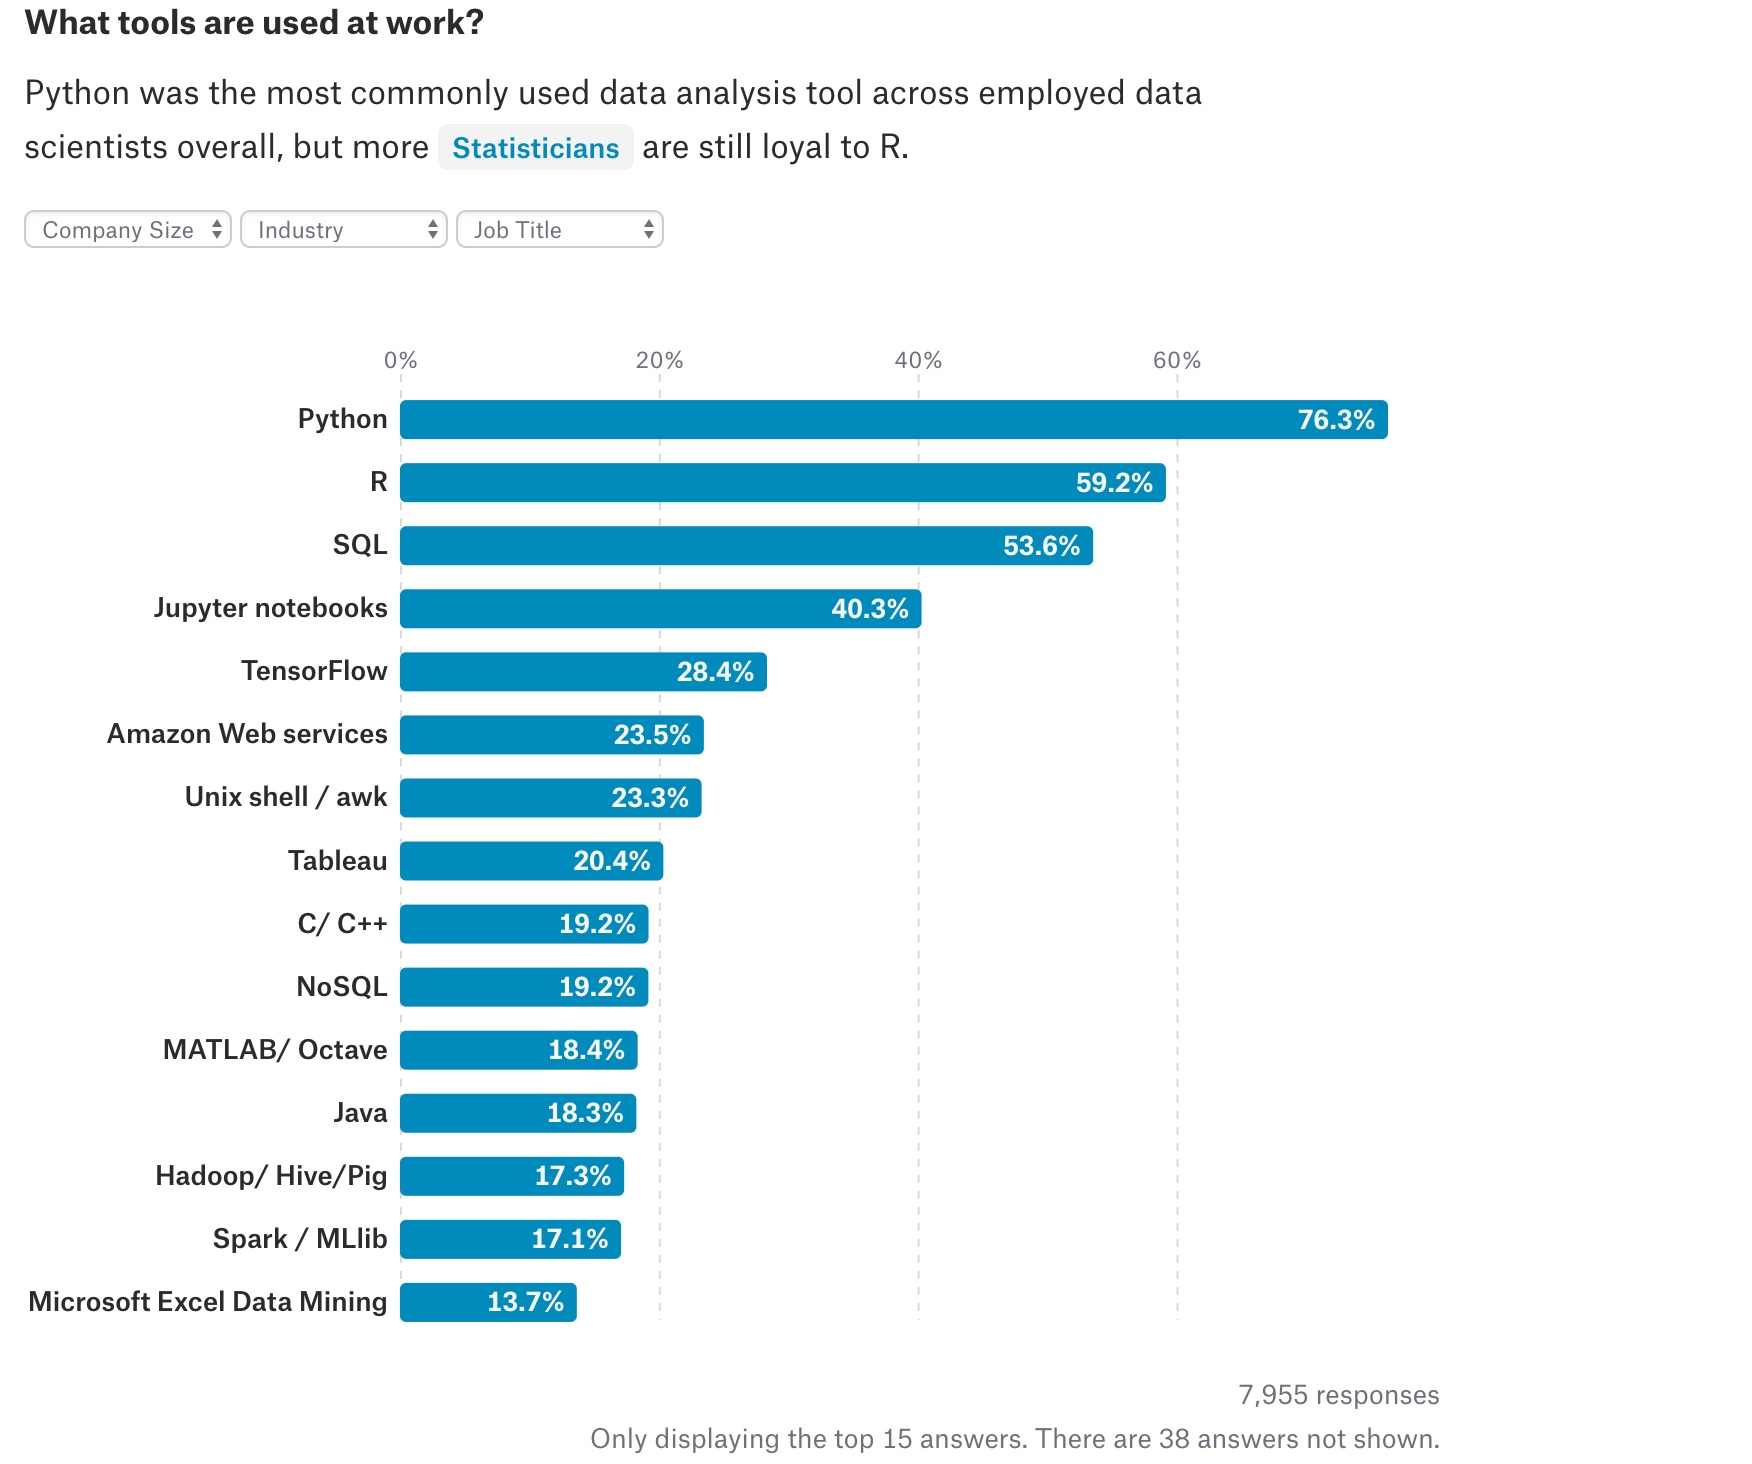
\includegraphics[width = 10 cm]{./viz/ext/Kaggle_DS_Tools_Survey.jpeg}
    \end{figure}

\begin{minipage}[ht]{0.2\linewidth}
    
\includegraphics[width=2\baselineskip]{./viz/icons/Think.png}  
\end{minipage}%
\begin{minipage}[ht]{0.75\linewidth}
\emph{Think like an Analyst:} Criticize the plots in terms of their inadequacy to provide the complete information. Argue, why and how would this lead to drawing of incorrect conclusions. 
\end{minipage}

\begin{minipage}[ht]{0.2\linewidth}
    
\includegraphics[width=2\baselineskip]{./viz/icons/Homework.png}  
\end{minipage}%
\begin{minipage}[ht]{0.75\linewidth}
Read the reports
\begin{enumerate}
  \item \textbf{``Eupopean Data Science Salary Survey''} published by O'REILLY in 2017
  \item \textbf{``The State of Data Science \& Machine Learning''} published by Kaggle in 2017
\end{enumerate}
and get yourself acquainted with \emph{stage 5} of the data exploration process.
\end{minipage}

%================================  
\subsection{A Brief History of R}
%================================
\textcolor{yellow}{TODO}
%================================
\subsection{Concepts for Programming with R}
%================================
%================================
\subsubsection{Functional Programming}
%================================
\begin{mdframed}[backgroundcolor=cyan!10]
\par\noindent{
Software in R is written in a \emph{functional style} that 
emphasizes on \emph{encapsulating computations via functions} thereby allowing the programmer to create \emph{abstractions by separating behaviour from implementation}.}
\end{mdframed}

\begin{minipage}[ht]{0.2\linewidth}
    
\includegraphics[width=2\baselineskip]{./viz/icons/Think.png}  
\end{minipage}%
\begin{minipage}[ht]{0.75\linewidth}
If you are given a set of $N$ numbers whose average needs to be computed, think about how would the functional programming approach allow you to achieve abstraction and what would be its benefit?
\emph{Hint:} Think about how would the computation of average differ when $N$ numbers are given in one go (\textbf{\emph{batched input}}) as opposed to when you get every number one after the other (\textbf{\emph{streaming input}})
\end{minipage}

%================================
\subsubsection{Classes and Methods}
%================================
\begin{mdframed}[backgroundcolor=cyan!10]
\par\noindent{
\emph{``Functions in R return objects'}'. Therefore any kind of \textbf{\emph{data in R is always an object}}. While functions facilitate abstraction by encapsulating implementation of computation, \emph{classes encapsulate objects}. \emph{Methods in R knit together functions and classes}.   
}
\end{mdframed}
%================================
\subsubsection{Data Frames}
%================================
\begin{mdframed}[backgroundcolor=cyan!10]
\par\noindent{
A \emph{data frame} is organization of data as observations (rows) and attributes (columns). Data frames are one of the predominant data structures in R. Moreover, they are synonymous with the tabular rebresentation of data as is found in spreadsheets and relational database systems. Such similarity in representation of data enables seamless integration between R and most spreadsheets and RDBMS systems. 
}
\end{mdframed}
%================================
\subsubsection{Ecosystem}
%================================
\begin{mdframed}[backgroundcolor=cyan!10]
\par\noindent{
R is an open-source software, thereby providing access to source code sufficient to generate a working version of the software. R is distributed under a version of GPL (Gnu Public License). An effect of this is that R has a thriving community of contributors and active users. Users, seek out existing implementation of data analysis/modeling techniques from a repository caled \textbf{\emph{CRAN}} (\textcolor{cyan}{\url{https://cran.r-project.org/}}). When they do not find an existing implementation that suits their needs, they create their own implementations, \emph{package} these implementations and contribute them back to CRAN. As a result of this CRAN today boasts a total of 12000+ packages. Please see the plot below that shows the growth in number of CRAN packages over time. This has resulted in R being unparalled in the number of options it provides for data analysis. Moreover, R is the primary tool used for statistical research (and has been so for 20 years). Therefore, when new methods are developed, they are not just published as a paper - they are also published as an R package. This means R is always on the cutting edge of new technologies. Furthermore, R was designed as an interface language - a means to present a consistent language interface for algorithms written in other languages. Many packages work by providing R language bindings to other open-source software, making R a convenient hub for all kinds of algorithms and methods.     
}
\end{mdframed}
\begin{figure}[ht] % Figure to demonstrate growth in number of CRAN packages over time
      \centering
      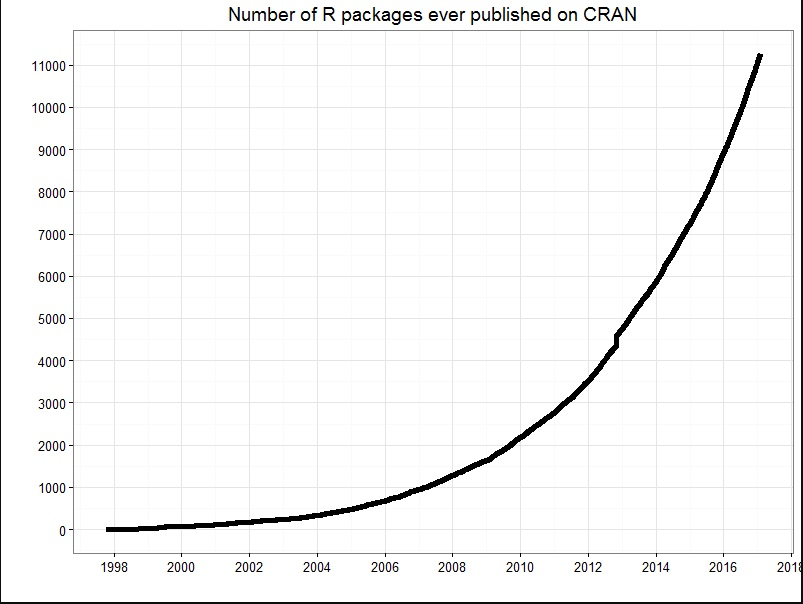
\includegraphics[width = 10 cm]{./viz/ext/numberofCRANpackages_over_Time.jpeg}
    \end{figure}

\begin{minipage}[ht]{0.2\linewidth}
    
\includegraphics[width=2\baselineskip]{./viz/icons/Think.png}  
\end{minipage}%
\begin{minipage}[ht]{0.75\linewidth}
Did you notice the sudden discontinuity in the curve around the year 2013? Can you think of what might have caused this?
\end{minipage}

\begin{minipage}[ht]{0.2\linewidth}
    
\includegraphics[width=2\baselineskip]{./viz/icons/Think.png}  
\end{minipage}%
\begin{minipage}[ht]{0.75\linewidth}
Argue \textbf{\emph{Why R}} statisfies \emph{the prime directives} and should therefore be our tool of choice for our mission of data exploration
\end{minipage}
    
\section{RStudio}
\begin{mdframed}[backgroundcolor=cyan!10]
\par\noindent{
\begin{minipage}[ht]{0.2\linewidth}
    
\includegraphics[width=2\baselineskip]{./viz/icons/Homework.png}  
\end{minipage}%
\begin{minipage}[ht]{0.75\linewidth}
Watch the video on \\
\textcolor{cyan}{\url{https://www.rstudio.com/resources/webinars/rstudio-essentials-webinar-series-part-1/}}\\
and install R and RStudio on the computer that you will be accessing during the sessions.
\end{minipage}
}
\end{mdframed}

\begin{minipage}[ht]{0.2\linewidth}
    
\includegraphics[width=2\baselineskip]{./viz/icons/Warning.png}  
\end{minipage}%
\begin{minipage}[ht]{0.75\linewidth}
\textcolor{red}{It is important that the participants have R and RStudio installed on their computers before Session 1.}
\end{minipage}

\begin{minipage}[ht]{0.2\linewidth}
    
\includegraphics[width=2\baselineskip]{./viz/icons/Homework.png}  
\end{minipage}%
\begin{minipage}[ht]{0.75\linewidth}
Download the RStudio IDE Cheat Sheet and use it as a reference while working with RStudio. In order to download the Cheat Sheet, \emph{Open RStudio > Go to  Help Menu > Cheatsheets > RStudio IDE Cheat Sheet} 
\end{minipage}

\section{Using R}
\begin{knitrout}
\definecolor{shadecolor}{rgb}{0.969, 0.969, 0.969}\color{fgcolor}\begin{kframe}
\begin{alltt}
\hlopt{?}\hlstd{View}
\end{alltt}
\end{kframe}
\end{knitrout}

\begin{knitrout}
\definecolor{shadecolor}{rgb}{0.969, 0.969, 0.969}\color{fgcolor}\begin{kframe}
\begin{alltt}
\hlkwd{help}\hlstd{(View)}
\end{alltt}
\end{kframe}
\end{knitrout}

